% RNAAS submission - A Label-Free Reliability Test for FR-I/FR-II Classification
%
% Limits (verified 2026-11-24 against journals.aas.org):
%   1,500 words INCLUDING title, headers, captions and references,
%   with 150 reserved for the required abstract.
%   One figure OR one table, not both.
%   Current draft: ~1,448 words. The AAS Editorial Office count is the final arbiter.
%
% Macros verified 2026-11-25 against the AASTeX v7.0 Author Guide
% (journals.aas.org/aastexguide/), CTAN v7.0.1 (2025-05-09), github.com/AASJournals/AASTeX7.
%
% VERIFIED CORRECT: \author[ORCID]{Name}; \affiliation{};
%   \keywords{\uat{Label}{id}} (label first, concept number second);
%   \apj \apjs \mnras \pasa; thebibliography with \bibitem[Author(Year)]{key}.
%
% CHANGED FROM v6.3, and fixed here:
%   - \email is now REQUIRED for every author/affiliation grouping; a missing one
%     stops the compile. One has been added below.
%   - \affil, \altaffilmark, \altaffiltext, \and are REMOVED in v7 and now error.
%   - \acknowledgments is removed; use the acknowledgments environment.
%   - Keywords must be alphabetical, maximum six. Reordered below.
%   - Section headings must be UPPER CASE for \section (mixed case for \subsection).
%     Five headings are used; they cost ~8 words against the 1,500 limit.
%
% NOT VERIFIED - check before submitting:
%   [ ] The [RNAAS] class option is NOT in the v7 style-option list (which is
%       twocolumn, preprint, preprint2, modern, manuscript, default, astrosymb,
%       tighten, times, linenumbers, trackchanges, longauthor, anonymous, longbib,
%       resetfootnotes, twocolappendix). It is omitted here rather than guessed at.
%       Confirm with the AAS editorial office how a Research Note is to be declared.
%   RESOLVED: the Overleaf AASTeX v7 template ships aastex701.cls, so the class is
%   loaded as {aastex701}, not {aastex7} as the guide writes. Set accordingly below.
%   [ ] LINE NUMBERS CONFLICT: the AASTeX guide calls \documentclass[linenumbers]
%       mandatory for submissions, but the RNAAS preparation guidelines say notes
%       must carry NO line numbers. RNAAS guidance is followed here. Confirm.
%   [ ] doi: inside \bibitem is not documented for v7; full DOI strings are
%       written out below instead.
%
% TODO: add the affiliation and email on lines below.

% Matches the file name shipped in the Overleaf AASTeX v7 template (aastex701.cls).
% To check whether an RNAAS option exists, search aastex701.cls for: RNAAS
\documentclass{aastex701}

\begin{document}

\title{A Label-Free Reliability Test for FR-I/FR-II Classification in Blind Radio Surveys}

\author[0009-0008-8798-2540]{Raj Kondekar}
\affiliation{Independent Researcher}
\email[show]{raj.kondekar@xaviers.edu.in}   % required in v7; compile stops without it

\begin{abstract}
Morphological classifiers trained on curated radio-galaxy samples are increasingly applied
to blind survey catalogues, where no labels exist to check them. We apply a five-seed
ResNet-18 ensemble trained on MiraBest to 1996 extended components from the FIRST catalogue,
and ask which label-free diagnostics detect a failed transfer. The candidate inputs are far
outside the training domain, with only 15\% falling inside MiraBest's angular-size range. The
predicted class changes under a rotation or mirror for 21.7\% (19.9--23.5\%) of candidates,
compared with 11.4\% (9.4--13.6\%) for MiraBest sources held out under five-fold
cross-validation. Restricting the candidates to MiraBest's size range, or to isolated
components, does not recover stability, so selection cannot repair the transfer. Ensemble
seed disagreement fails as a diagnostic once it is referenced against a properly powered
baseline. We recommend dihedral instability as a per-source reliability score for survey
pipelines.
\end{abstract}

% UAT concepts verified 2026-11-25 against the official vocabulary file
% (raw.githubusercontent.com/astrothesaurus/UAT/master/UAT_list.json, release 6.0.0),
% parsed locally rather than taken from a search page.
% Alphabetical order is required; maximum six.
\keywords{\uat{Astronomy data analysis}{1858} ---
          \uat{Convolutional neural networks}{1938} ---
          \uat{Extragalactic radio sources}{508} ---
          \uat{Fanaroff-Riley radio galaxies}{526}}

\section{INTRODUCTION}

The Evolutionary Map of the Universe is expected to catalogue about 70 million radio
galaxies \citep{norris2011}, far more than can be inspected by eye, and convolutional neural
networks are now a standard tool for classifying them \citep{aniyan2017}. Fanaroff--Riley
type separates sources by whether their emission peaks near the core or the edges, a
division that correlates with radio luminosity \citep{fanaroff1974}, so FR demographics at
survey scale bear on jet power and environment. That use depends on the classifications
being meaningful for the sources the classifier is actually given.

Training sets do not look like survey catalogues. Labelled sets such as MiraBest
\citep{porter2023} are curated: the sources are extended, centred on their host, and were
chosen because a human could classify them confidently. A blind catalogue is none of these
things. Its rows are components rather than whole sources, most are barely resolved, and
many are not FR galaxies at all. A classifier still returns a confident-looking probability
for every row.

Standard validation does not reveal this. Held-out accuracy is measured on sources from the
same curated distribution, so it says nothing about behaviour on sources unlike them, and
blind samples have no labels at all. A survey pipeline instead needs a diagnostic that can
be computed without labels, for each source, and that flags when an output should not be
trusted. We test two such diagnostics, and whether simple selection cuts can fix the problem
instead.

\section{DATA AND METHOD}

We selected 1996 extended components from the FIRST catalogue
\citep{becker1995,helfand2015}, taking every 94th of the 946,432 entries and keeping those
with an integrated-to-peak flux ratio above 1.25, a deconvolved major axis above
$6''$, and a signal-to-noise ratio above 7. We discarded cutouts with missing pixels and
components within $30''$ of a MiraBest position. The images are $4.5'$ SkyView cutouts
\citep{mcglynn1998} at the native $1.8''$ pixel scale, giving $150 \times 150$ pixels,
matching MiraBest's format. Each is background-subtracted, thresholded at $3\sigma$, and
scaled to unit maximum.

The classifier is an ensemble of five ResNet-18 networks \citep{he2016} trained on
MiraBest's 729 confident sources with full eight-fold dihedral augmentation, keeping
final-epoch weights so no model was selected on the data it is evaluated against.

The diagnostic itself is simple. A radio galaxy has no preferred orientation, so a
classifier's answer should not depend on how the image is rotated or mirrored, and
group-equivariant networks build this invariance in by design \citep{scaife2021}. We call a
source unstable if the ensemble-mean predicted class is not the same across all eight
symmetries of the square. The measurement needs no label and costs eight forward passes.

An instability rate means little without a baseline, and one taken from a small held-out set
is too noisy to serve. We therefore ran five-fold cross-validation over all 833 confident
MiraBest sources, giving every source a prediction from models that never saw it. This
raises the reference from 104 sources to 833, with a held-out accuracy of 91.2\%
(89.1--93.0\%).

One check underpins the comparison. Passing the 104 held-out galaxies through our own cutout
and preprocessing path, rather than their native images, changed little: 99.0\% label
agreement and a median probability difference of 0.004. The instability below is therefore a
property of the candidate sample, not of our pipeline.

\section{RESULTS}

The candidate sample lies well outside the training domain. Only 15.3\% (13.8--16.9\%) fall
inside MiraBest's 10th-to-90th-percentile angular-size range, and MiraBest's 10th percentile
exceeds the candidates' 75th. Measured on the pixels with identical preprocessing, the
median candidate spans $18.0''$ against MiraBest's $41.4''$, with 123 pixels above threshold
against 294.5.

Instability follows that distance. The predicted class changes under a rotation or mirror
for 21.7\% (19.9--23.5\%) of candidates, compared with 11.4\% (9.4--13.6\%) for the
cross-validated MiraBest reference. The gap is 10.3 percentage points, the intervals do not
overlap, and the candidate rate is 1.9 times the reference. We had set a threshold of 10
points in advance, so the result clears it by only 0.3 points. The effect is real, but the
margin is narrow, and a larger candidate sample would test it more strongly.

The ordering across cohorts is the clearest form of the result (Figure~\ref{fig:ladder}).
The flip rate rises steadily with distance from the training set: 1.8\% on the training
sources, 11.4\% on held-out MiraBest sources, 21.7\% on blind FIRST candidates, 24.2\% on
MiraBest's uncertain class, and 41.2\% on its hybrids. The blind sample sits next to the
sources MiraBest itself could not classify, rather than next to the sources the classifier
handles well.

Selection does not repair the problem. Restricting the candidates to MiraBest's angular-size
range leaves the flip rate at 23.2\% using the catalogue's deconvolved axis, or 22.8\% using
the pixel extent, both slightly worse than the unrestricted sample. Two thirds (68.6\%) have
another catalogued component within $2.25'$, and keeping only the isolated ones gives
17.1\%, still 1.5 times the reference. None of the cuts a survey pipeline would naturally
apply returns the sample to baseline.

Not every diagnostic works. Seed disagreement separates the samples by only 3.7 points,
41.8\% against 38.2\%, with overlapping intervals. Against a 104-source reference it had
seemed to miss our threshold by 0.4 points; properly powered, the baseline is 38.2\%, not
15.4\%. It is not a usable reliability score.

\section{DISCUSSION}

Because no selection cut restores stability, reliability must be assessed per source rather
than per sample. We suggest that pipelines applying morphology classifiers to blind
catalogues report each source's dihedral instability alongside its class, and treat unstable
sources as unclassified rather than as low-confidence members of a class.

We offer one interpretation of the ordering, which no test here demonstrates. It is
consistent with a blind sample posing a different problem rather than a harder version of
the same one: many rows may have no true FR class, and a two-class classifier asked about
such a source can only answer unstably. Testing this needs labels for a blind subsample, or
a third class.

Three limits apply. The candidates are scored by the published ensemble while the reference
comes from the cross-validation models, so the comparison is between two model sets trained
the same way rather than identical weights. The diagnostic has been tested on one survey,
one architecture and one training set. It also assumes a classifier that is not equivariant
by construction: a group-equivariant network would show almost no flips by design, removing
the symptom rather than the domain shift, and with it a free reliability signal.

\section{DATA AVAILABILITY}

Code, pre-registered criteria and all reported numbers are at
\url{https://github.com/astrophile73/radio-astronomy-ml-morphology}; weights and cached
predictions are deposited at \url{https://doi.org/10.5281/zenodo.24497097}.

\begin{figure}[ht!]
\centering
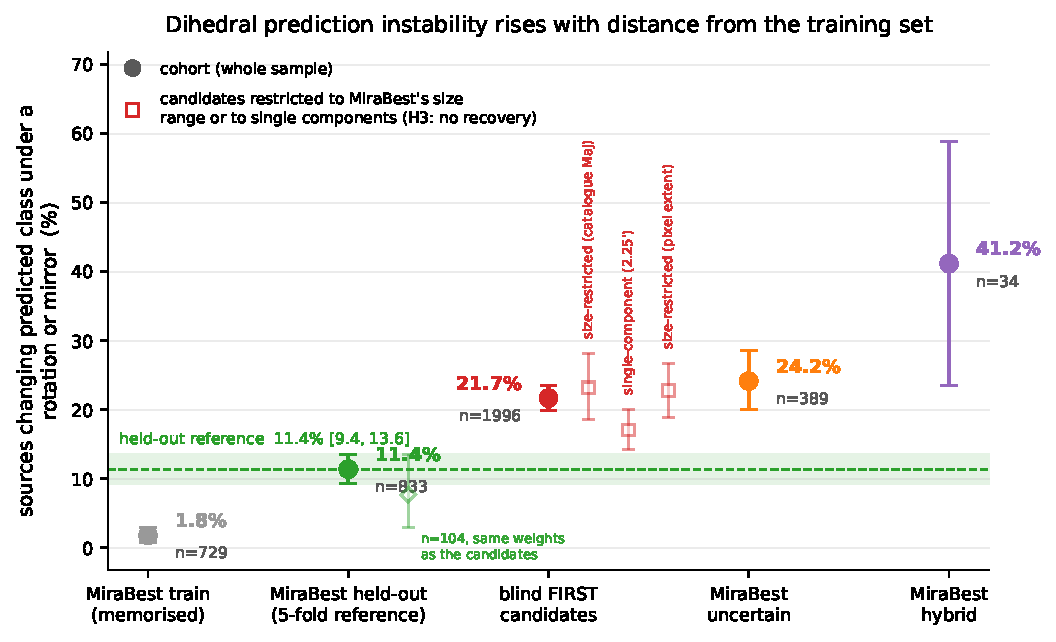
\includegraphics[width=\linewidth]{fig1_flip_rate_ladder.pdf}
\caption{Dihedral instability, the fraction of sources whose predicted class changes under
at least one of the eight rotations and mirrors of the square, for five cohorts ordered by
distance from the training set. Error bars are bootstrap 95\% intervals and the shaded band
is the five-fold held-out MiraBest reference. Open squares show candidates restricted to
MiraBest's angular-size range or to isolated components; none returns to baseline.
\label{fig:ladder}}
\end{figure}

\begin{thebibliography}{}

\bibitem[Aniyan \& Thorat(2017)]{aniyan2017} Aniyan, A.~K., \& Thorat, K. 2017, \apjs, 230,
20, doi:10.3847/1538-4365/aa7333

\bibitem[Becker et al.(1995)]{becker1995} Becker, R.~H., White, R.~L., \& Helfand, D.~J.
1995, \apj, 450, 559, doi:10.1086/176166

\bibitem[Fanaroff \& Riley(1974)]{fanaroff1974} Fanaroff, B.~L., \& Riley, J.~M. 1974,
\mnras, 167, 31P, doi:10.1093/mnras/167.1.31P

\bibitem[He et al.(2016)]{he2016} He, K., Zhang, X., Ren, S., \& Sun, J. 2016, in Proc. IEEE
CVPR, 770, doi:10.1109/CVPR.2016.90

\bibitem[Helfand et al.(2015)]{helfand2015} Helfand, D.~J., White, R.~L., \& Becker, R.~H.
2015, \apj, 801, 26, doi:10.1088/0004-637X/801/1/26

\bibitem[McGlynn et al.(1998)]{mcglynn1998} McGlynn, T., Scollick, K., \& White, N. 1998, in
IAU Symp. 179, New Horizons from Multi-Wavelength Sky Surveys, 465

\bibitem[Norris et al.(2011)]{norris2011} Norris, R.~P., Hopkins, A.~M., Afonso, J., et al.
2011, \pasa, 28, 215, doi:10.1071/AS11021

\bibitem[Porter \& Scaife(2023)]{porter2023} Porter, F.~A.~M., \& Scaife, A.~M.~M. 2023,
RAS Techniques and Instruments, 2, 293, doi:10.1093/rasti/rzad017

\bibitem[Scaife \& Porter(2021)]{scaife2021} Scaife, A.~M.~M., \& Porter, F. 2021, \mnras,
503, 2369, doi:10.1093/mnras/stab530

\end{thebibliography}

\end{document}
